\documentclass[11pt]{article}

\usepackage[utf8]{inputenc}
\usepackage[T1]{fontenc}
\usepackage[french]{babel}
\usepackage{amsmath, amssymb}
\usepackage{graphicx}
\usepackage{geometry}
\usepackage{booktabs}
\usepackage{tikz}
\usepackage{caption}
\usetikzlibrary{positioning, arrows.meta}

\geometry{margin=2.5cm}

\title{Cybernet IA : Détection d’attaques dans les réseaux SDN par apprentissage automatique }
\author{Belhoussine Jihane \and Tulliez Paul \and Viviès Clémence}
\date{}

\begin{document}

\maketitle


\begin{abstract}
Les réseaux définis par logiciel (SDN) offrent une grande flexibilité grâce à la séparation des plans de contrôle et de données, mais cette centralisation introduit des vulnérabilités critiques, notamment face aux attaques ciblant le contrôleur. En particulier, les attaques par déni de service et les surcharges de type \textit{Packet-In} peuvent compromettre la disponibilité du réseau en saturant le plan de contrôle.

Dans cet article, nous proposons \textit{Cybernet IA}, un système de détection d’intrusions dédié aux environnements SDN, reposant sur un modèle d’apprentissage supervisé de type Random Forest. L’approche s’appuie sur une architecture expérimentale complète intégrant Mininet, Open vSwitch et le contrôleur Ryu, permettant la génération de scénarios réalistes de trafic normal et malveillant ainsi que la collecte et la labellisation automatique des données.

Nous introduisons un pipeline de bout en bout couvrant l’extraction de caractéristiques via OpenFlow, le prétraitement des données et l’entraînement du modèle. L’évaluation expérimentale, réalisée sur un jeu de données représentatif comprenant plusieurs types d’attaques, montre que le modèle atteint une précision et un rappel équilibrés autour de 83\%, démontrant sa capacité à détecter efficacement des comportements anormaux à partir de caractéristiques statistiques simples.

Enfin, nous discutons les limites de l’approche et proposons des perspectives d’évolution vers une détection en temps réel en flux continu, adaptée aux contraintes des environnements SDN opérationnels.
\end{abstract}



\section{Introduction}

La transformation numérique des infrastructures informatiques a conduit à l’émergence de paradigmes réseaux plus flexibles, programmables et dynamiques. Dans ce contexte, les réseaux définis par logiciel (\textit{Software-Defined Networking}, SDN) se sont imposés comme une architecture de référence, reposant sur la dissociation entre le plan de contrôle et le plan de données. Cette séparation permet une gestion centralisée du réseau via un contrôleur logiciel, facilitant l’orchestration, l’automatisation et l’adaptation dynamique des politiques réseau.

Cependant, cette centralisation introduit également de nouveaux défis en matière de sécurité. En particulier, le contrôleur SDN constitue un point critique du système, souvent qualifié de \textit{Single Point of Failure}. Des attaques ciblant le plan de contrôle, telles que les attaques par déni de service distribué (DDoS) ou les surcharges de type \textit{Packet-In}, peuvent rapidement saturer les ressources du contrôleur et compromettre le fonctionnement global du réseau. Ces vulnérabilités sont d’autant plus critiques dans des environnements à forte densité de trafic, tels que les centres de données ou les infrastructures cloud.

Les approches traditionnelles de détection d’intrusions, principalement fondées sur des signatures, montrent leurs limites face à la complexité et à la variabilité des attaques modernes. Elles nécessitent une mise à jour constante des bases de signatures et peinent à détecter des comportements inconnus ou évolutifs. Dans ce contexte, les techniques d’apprentissage automatique apparaissent comme une alternative prometteuse, permettant de modéliser le comportement normal du réseau et de détecter automatiquement des anomalies à partir de caractéristiques statistiques du trafic.

Néanmoins, plusieurs défis subsistent dans l’intégration de ces approches au sein des architectures SDN. D’une part, les contraintes de temps réel et de performance imposent l’utilisation de modèles légers, capables de produire des prédictions rapides directement au niveau du contrôleur. D’autre part, la disponibilité de jeux de données adaptés, représentatifs des spécificités des réseaux SDN, constitue un obstacle majeur à l’évaluation et à la comparaison des méthodes proposées.

Dans ce contexte, cet article propose \textit{Cybernet IA}, un système de détection d’intrusions conçu pour les environnements SDN, reposant sur un algorithme de classification Random Forest. Contrairement à des approches plus complexes basées sur des architectures profondes, notre choix s’inscrit dans une démarche pragmatique visant à concilier efficacité de détection et coût computationnel réduit, afin de permettre une intégration opérationnelle au sein du contrôleur réseau.

L’une des originalités de ce travail réside dans la conception d’un environnement expérimental complet et reproductible, basé sur Mininet, Open vSwitch et le contrôleur Ryu. Cet environnement permet de générer dynamiquement des scénarios de trafic réalistes, incluant à la fois des flux légitimes et plusieurs types d’attaques, tout en assurant une labellisation automatique des données collectées. Il constitue ainsi un cadre cohérent pour l’entraînement et l’évaluation de modèles d’apprentissage automatique appliqués à la sécurité des réseaux SDN.

Plus précisément, les contributions de cet article sont les suivantes. Premièrement, nous proposons une architecture modulaire de collecte et de traitement de données réseau reposant sur les mécanismes natifs du protocole OpenFlow. Deuxièmement, nous développons un pipeline complet de génération de données, de prétraitement et d’apprentissage supervisé, permettant la construction d’un modèle de détection robuste à partir de caractéristiques statistiques des flux. Troisièmement, nous réalisons une évaluation expérimentale approfondie du modèle Random Forest sur un ensemble de scénarios d’attaque variés, mettant en évidence ses performances et ses limites. Enfin, nous discutons les perspectives d’évolution vers une détection en temps réel en flux continu, adaptée aux contraintes opérationnelles des environnements SDN.

Le reste de l’article est organisé comme suit. La Section~\ref{sec:related_work} présente les travaux connexes relatifs à la détection d’intrusions en environnement SDN. La Section~\ref{sec:architecture} décrit l’architecture du système proposé. La Section~\ref{sec:methodology} détaille la méthodologie adoptée pour la collecte et le traitement des données ainsi que l’entraînement du modèle. Les résultats expérimentaux et leur analyse sont présentés dans la Section~\ref{sec:results}. Enfin, la Section~\ref{sec:conclusion} conclut l’article et ouvre des perspectives de recherche.
\section{Préliminaires}

Afin de faciliter la compréhension des contributions proposées dans cet article, cette section rappelle brièvement les notions fondamentales relatives aux réseaux définis par logiciel (SDN), au protocole OpenFlow, ainsi qu’aux principes généraux de l’apprentissage automatique appliqué à la détection d’intrusions.

\subsection{Réseaux définis par logiciel (SDN)}

Les réseaux définis par logiciel (\textit{Software-Defined Networking}, SDN) constituent une architecture réseau dans laquelle le plan de contrôle est dissocié du plan de données. Cette séparation permet de centraliser la logique de décision dans un contrôleur, tandis que les équipements de commutation se limitent à l’acheminement des paquets selon des règles installées dynamiquement.

Le modèle SDN repose généralement sur trois couches principales :

\begin{itemize}
    \item le \textbf{plan de données}, composé de commutateurs programmables,
    \item le \textbf{plan de contrôle}, représenté par un contrôleur centralisé,
    \item la \textbf{couche applicative}, où s’exécutent les applications réseau (sécurité, routage, optimisation).
\end{itemize}

\subsection{Protocole OpenFlow}

OpenFlow est l’un des protocoles les plus utilisés pour la communication entre le contrôleur SDN et les commutateurs. Il permet au contrôleur d’installer, modifier ou supprimer des règles de flux dans les tables des commutateurs.

Lorsqu’un paquet ne correspond à aucune règle existante, un message \texttt{Packet-In} est envoyé au contrôleur. Celui-ci prend alors une décision et peut répondre via un message \texttt{Flow-Mod}, afin d’installer une règle appropriée. Ce mécanisme constitue le cœur de la programmabilité SDN, mais introduit également des vulnérabilités exploitables par des attaques de type surcharge.

\subsection{Apprentissage automatique pour la détection d’intrusions}

La détection d’intrusions basée sur l’apprentissage automatique consiste à apprendre un modèle capable de distinguer le trafic normal du trafic malveillant à partir de caractéristiques observables du réseau.

Dans un cadre supervisé, le système apprend une fonction de classification à partir d’un ensemble d’exemples labellisés. Les modèles les plus couramment utilisés incluent les arbres de décision, les forêts aléatoires, les machines à vecteurs de support et les réseaux de neurones.

Dans le contexte SDN, ces modèles sont généralement alimentés par des caractéristiques agrégées issues du plan de contrôle, telles que le nombre de paquets, le volume de données ou la durée des flux.
\subsection{Forêts aléatoires (Random Forest)}

La forêt aléatoire (\textit{Random Forest}) est une méthode d’apprentissage supervisé appartenant à la famille des méthodes d’ensemble (\textit{ensemble learning}). Elle repose sur la construction d’un ensemble d’arbres de décision entraînés de manière indépendante, puis agrégés afin de produire une prédiction finale robuste.

Chaque arbre est construit à partir d’un échantillonnage aléatoire des données d’entraînement (technique de \textit{bootstrap}) ainsi que d’un sous-ensemble aléatoire de variables à chaque division de nœud. Cette double randomisation permet de réduire la corrélation entre les arbres et d’améliorer la capacité de généralisation du modèle.

Formellement, étant donné un ensemble de $K$ arbres $\{T_k\}_{k=1}^{K}$, la prédiction finale pour un vecteur de caractéristiques $\mathbf{x}$ est obtenue par vote majoritaire :

\begin{equation}
\hat{y} = \mathrm{mode} \left( T_1(\mathbf{x}), T_2(\mathbf{x}), \dots, T_K(\mathbf{x}) \right)
\end{equation}

Dans le cas d’une classification probabiliste, la décision peut également être exprimée comme la moyenne des probabilités prédites par chaque arbre :

\begin{equation}
P(y=1 \mid \mathbf{x}) = \frac{1}{K} \sum_{k=1}^{K} P_k(y=1 \mid \mathbf{x})
\end{equation}

Les forêts aléatoires présentent plusieurs avantages particulièrement adaptés aux environnements SDN :

\begin{itemize}
    \item \textbf{Robustesse au surapprentissage} grâce à l’agrégation de multiples modèles,
    \item \textbf{Faible coût d’inférence}, compatible avec des contraintes temps réel,
    \item \textbf{Capacité à modéliser des relations non linéaires} entre les caractéristiques,
    \item \textbf{Bonne interprétabilité relative} via l’analyse de l’importance des variables.
\end{itemize}

Dans le contexte de la détection d’intrusions, ce modèle est particulièrement pertinent car il permet de capturer des interactions complexes entre les métriques réseau (débit, durée, volume) tout en conservant une latence d’exécution faible, ce qui facilite son intégration directe dans le plan de contrôle SDN.

Enfin, les forêts aléatoires fournissent également des mesures d’importance des variables (\textit{feature importance}), qui permettent d’identifier les caractéristiques les plus discriminantes pour la détection des attaques, ce qui constitue un outil précieux pour l’analyse du comportement du modèle.

\subsection{Vue conceptuelle du système}

La figure suivante illustre de manière simplifiée l’interaction entre les couches SDN et le module d’apprentissage automatique intégré dans le contrôleur.

\begin{figure}[h]
\centering
\begin{tikzpicture}[
    node distance=1.8cm,
    block/.style={draw, rectangle, rounded corners, align=center, minimum width=3.6cm, minimum height=1cm},
    arrow/.style={->, thick}
]

% Layers
\node[block] (data) {Plan de données\\(Switches OpenFlow)};
\node[block, above=of data] (control) {Plan de contrôle\\(SDN Controller)};
\node[block, above=of control] (ml) {Module IA\\(Random Forest IDS)};

\node[block, right=4cm of control] (app) {Applications réseau\\(Sécurité, routage, etc.)};

% Arrows
\draw[arrow] (data) -- (control);
\draw[arrow] (control) -- (data);

\draw[arrow] (control) -- (ml);
\draw[arrow] (ml) -- (control);

\draw[arrow] (control) -- (app);

\end{tikzpicture}
\caption{Architecture conceptuelle SDN avec intégration d’un module de détection basé sur l’apprentissage automatique}
\end{figure}

\medskip

Ces préliminaires fournissent les bases nécessaires pour comprendre l’architecture et la méthodologie proposées dans la suite de l’article, notamment l’intégration d’un modèle d’apprentissage automatique au sein du contrôleur SDN pour la détection d’intrusions en temps réel.

\section{Modèle de menace}

Le modèle de menace considéré dans ce travail s’inscrit dans le contexte d’un réseau SDN où le plan de contrôle est centralisé et accessible via le protocole OpenFlow. Cette centralisation, bien qu’avantageuse en termes de flexibilité et de programmabilité, constitue une surface d’attaque privilégiée pour des adversaires cherchant à perturber le fonctionnement global du réseau.

Nous considérons un attaquant disposant d’un accès au plan de données, typiquement sous la forme d’un ou plusieurs hôtes compromis au sein du réseau. Cet attaquant est capable de générer du trafic arbitraire, en modulant à la fois le volume, la fréquence et les caractéristiques des flux. Il ne dispose pas d’un accès direct au contrôleur, mais exploite les mécanismes standards du protocole OpenFlow pour provoquer une surcharge indirecte.

L’objectif principal de l’attaquant est de dégrader la disponibilité du contrôleur SDN en exploitant le mécanisme de gestion des flux inconnus. En générant un grand nombre de paquets appartenant à des flux non encore installés dans les tables des commutateurs, l’attaquant force ces derniers à transmettre des messages \texttt{Packet-In} au contrôleur. Ce phénomène peut conduire à une saturation des ressources CPU et mémoire du contrôleur, entraînant une augmentation de la latence, voire une interruption du service.

Les scénarios d’attaque considérés incluent des attaques volumétriques classiques, telles que les TCP SYN Flood, les ICMP Flood et les UDP Flood, ainsi que des attaques plus spécifiques aux environnements SDN, comme la saturation des tables de flux (\textit{flow table overflow}) et les attaques visant à maximiser le nombre de requêtes \texttt{Packet-In}. Ces attaques partagent une caractéristique commune : elles induisent des motifs statistiques anormaux dans les flux réseau, exploitables par des méthodes d’apprentissage automatique.

Dans ce cadre, le système proposé ne repose sur aucune connaissance a priori des signatures d’attaque. Il adopte une approche comportementale, visant à distinguer le trafic légitime du trafic malveillant à partir de caractéristiques agrégées des flux. Cette hypothèse rend le système potentiellement plus robuste face à des attaques inconnues, tout en introduisant des défis en termes de généralisation.

Enfin, nous supposons que les mécanismes de collecte de statistiques via OpenFlow sont fiables et que les données observées ne sont pas altérées par l’attaquant. Cette hypothèse est classique dans les travaux sur la détection d’intrusions en SDN, bien qu’elle puisse être remise en question dans des scénarios d’attaque plus avancés impliquant une compromission du plan de contrôle.



\section{Travaux connexes}\label{sec:related_work}

La détection d’intrusions dans les réseaux définis par logiciel (SDN) constitue un domaine de recherche actif, à l’intersection de la sécurité des réseaux et de l’apprentissage automatique. La centralisation du plan de contrôle offre un point d’observation privilégié, permettant d’extraire des statistiques globales du trafic, mais elle impose également des contraintes fortes en termes de latence et de charge computationnelle.

Les premières approches de détection dans les environnements SDN reposaient principalement sur des méthodes à base de signatures ou de règles statiques. Bien que simples à mettre en œuvre, ces approches présentent des limites importantes face à l’évolution rapide des attaques, notamment leur incapacité à détecter des comportements inconnus ou polymorphes. Cette limitation a conduit à l’émergence de méthodes basées sur l’apprentissage automatique.

Parmi ces méthodes, les approches fondées sur le \textit{deep learning} ont suscité un intérêt croissant. Par exemple, Tang et al. \cite{ref1} proposent une architecture hybride combinant réseaux de neurones convolutifs (CNN) et réseaux récurrents de type LSTM pour capturer à la fois les dépendances spatiales et temporelles du trafic réseau. De même, certaines études exploitent des architectures profondes pour modéliser des séquences de flux et détecter des anomalies complexes. Bien que ces approches atteignent généralement des performances élevées, leur coût computationnel et leur latence d’inférence les rendent difficilement compatibles avec une intégration directe dans le contrôleur SDN, en particulier dans des environnements contraints.

En parallèle, plusieurs travaux ont exploré des modèles d’apprentissage plus légers, mieux adaptés aux contraintes opérationnelles. Les machines à vecteurs de support (SVM) ont été largement utilisées pour la détection d’anomalies dans les réseaux, notamment en raison de leur capacité à gérer des espaces de grande dimension. Toutefois, leur sensibilité au choix des hyperparamètres et leur difficulté à passer à l’échelle limitent leur utilisation dans des contextes de trafic massif. Les méthodes basées sur les plus proches voisins (KNN), bien que simples, souffrent quant à elles d’un coût de calcul élevé en phase d’inférence.

Les approches basées sur les arbres de décision et les méthodes d’ensemble constituent une alternative particulièrement pertinente. Dans ce contexte, les forêts aléatoires (\textit{Random Forest}) ont été largement étudiées pour la détection d’attaques de type DDoS dans les réseaux SDN. Comme le montrent les travaux récents présentés dans \cite{ref4}, ces modèles offrent un compromis efficace entre précision, robustesse et coût computationnel. Leur capacité à capturer des interactions non linéaires entre les variables, tout en limitant le surapprentissage, en fait des candidats adaptés à une intégration dans le plan de contrôle.

Par ailleurs, plusieurs études se sont intéressées spécifiquement aux attaques ciblant les mécanismes internes du SDN. L’analyse proposée dans \cite{ref2} met en évidence différentes stratégies d’attaque exploitant la gestion des flux et la communication entre le plan de données et le contrôleur. De même, les travaux de \cite{ref3} se concentrent sur les attaques dites « low and slow », qui visent à contourner les mécanismes de détection classiques en adoptant un comportement plus discret.

Au-delà des modèles eux-mêmes, la question de la qualité et de la représentativité des données d’entraînement constitue un enjeu central. De nombreux travaux s’appuient sur des datasets standardisés, tels que CICIDS2017 \cite{cicids}, qui offrent une grande diversité de scénarios d’attaque. Cependant, ces datasets ne reflètent pas toujours fidèlement les spécificités des environnements SDN, notamment en termes de métriques disponibles via OpenFlow. Cette limitation justifie le développement d’environnements expérimentaux dédiés, capables de générer des données adaptées au contexte étudié.

Dans cette perspective, notre approche se distingue par la combinaison de trois éléments. Premièrement, elle repose sur un modèle Random Forest, choisi pour son compromis entre performance et complexité. Deuxièmement, elle s’appuie sur une plateforme expérimentale reproductible permettant de générer des données réalistes dans un environnement SDN contrôlé. Enfin, elle adopte une approche centrée sur des caractéristiques directement extraites du plan de contrôle, facilitant ainsi une intégration potentielle en conditions opérationnelles.

Ce positionnement permet de combler le fossé entre les approches théoriques à haute performance mais peu déployables, et les solutions légères mais souvent limitées en termes de précision et de robustesse.



\section{Architecture du système}\label{sec:architecture}

Cette section décrit l’architecture globale de \textit{Cybernet IA}, en mettant en évidence les différents composants du système ainsi que leurs interactions. L’objectif est de proposer une chaîne de traitement complète, allant de la collecte des données réseau jusqu’à la détection d’anomalies, tout en assurant une intégration réaliste dans un environnement SDN.

\subsection{Vue d’ensemble}

L’architecture repose sur une séparation claire entre trois couches fonctionnelles : (i) le plan de données, (ii) le plan de contrôle, et (iii) la couche d’analyse intelligente. Cette organisation permet de préserver les principes fondamentaux du SDN tout en enrichissant le contrôleur avec des capacités d’analyse avancées.

\begin{figure}[h]
\centering
\begin{tikzpicture}[
    node distance=2cm,
    every node/.style={draw, rectangle, rounded corners, align=center, minimum width=3cm, minimum height=1cm},
    arrow/.style={->, thick}
]

% Nodes
\node (hosts) {Hôtes};
\node (switch) [below of=hosts] {Commutateurs\\(Open vSwitch)};
\node (controller) [below of=switch] {Contrôleur SDN\\(Ryu)};
\node (collector) [right of=controller, xshift=4cm] {Collecte\\Statistiques};
\node (ml) [below of=collector] {Modèle ML\\(Random Forest)};
\node (decision) [below of=controller] {Décision\\(IDS)};

% Arrows
\draw[arrow] (hosts) -- (switch);
\draw[arrow] (switch) -- (controller);
\draw[arrow] (controller) -- (switch);

\draw[arrow] (controller) -- (collector);
\draw[arrow] (collector) -- (ml);
\draw[arrow] (ml) -- (decision);
\draw[arrow] (decision) -- (controller);

\end{tikzpicture}
\caption{Architecture globale du système Cybernet IA}
\end{figure}

Comme illustré dans la Figure~1, le système s’insère directement dans la boucle de contrôle SDN. Le contrôleur joue un rôle central en assurant à la fois la gestion du réseau et la collecte des données nécessaires à la détection.

\subsection{Plan de données}

Le plan de données est constitué de commutateurs Open vSwitch déployés dans l’environnement Mininet. Ces commutateurs exécutent les règles de forwarding installées par le contrôleur et remontent les paquets inconnus via des messages \texttt{Packet-In}.

Dans notre architecture, les commutateurs ne possèdent aucune logique de sécurité avancée. Cette conception volontairement simple permet de centraliser l’intelligence au niveau du contrôleur, conformément au paradigme SDN.

\subsection{Plan de contrôle}

Le contrôleur Ryu constitue le cœur du système. Il assure plusieurs fonctions critiques :

\begin{itemize}
    \item apprentissage des adresses MAC (fonction de switch L2),
    \item installation dynamique des règles de flux,
    \item collecte périodique des statistiques via OpenFlow,
    \item interaction avec le module de détection.
\end{itemize}

La collecte des statistiques repose sur l’envoi de requêtes \texttt{OFPFlowStatsRequest} à intervalles réguliers. Ces requêtes permettent d’extraire des informations agrégées sur les flux actifs, sans nécessiter une inspection profonde des paquets.

\subsection{Pipeline de traitement des données}

Le pipeline de traitement constitue un élément clé de l’architecture. Il transforme les statistiques brutes en entrées exploitables par le modèle d’apprentissage automatique.

\begin{figure}[h]
\centering
\noindent\resizebox{\textwidth}{!}{
\begin{tikzpicture}[
    every node/.style={
        draw,
        rectangle,
        rounded corners,
        align=center,
        minimum width=3cm,
        minimum height=1cm
    },
    arrow/.style={
        ->,
        thick
    }
]

% Nodes
\node (collect) 
{Collecte\\(OpenFlow)};

\node (clean) [right=2.8cm of collect] 
{Nettoyage};

\node (norm) [right=2.8cm of clean] 
{Normalisation};

\node (model) [right=2.8cm of norm] 
{Modèle\\Random Forest};

\node (alert) [right=2.8cm of model] 
{Détection\\Alerte};

% Arrows
\draw[arrow] (collect) -- (clean);

\draw[arrow] (clean) -- (norm);

\draw[arrow] (norm) -- (model);

\draw[arrow] (model) -- (alert);

\end{tikzpicture}
}
\caption{Pipeline de traitement des données}

\end{figure}

Ce pipeline comprend quatre étapes principales :

Premièrement, les statistiques de flux sont collectées depuis le contrôleur. Deuxièmement, les données sont nettoyées afin de supprimer les attributs non pertinents. Troisièmement, une normalisation est appliquée pour homogénéiser les échelles. Enfin, les données sont injectées dans le modèle de classification.

\subsection{Module de détection et boucle de rétroaction}

Le modèle Random Forest produit une classification binaire (normal / attaque). Cette décision est ensuite exploitée par un module de détection qui peut déclencher différentes actions :

\begin{itemize}
    \item génération d’alertes,
    \item journalisation des événements,
    \item adaptation des règles de flux (mitigation).
\end{itemize}

Un point important de notre architecture est la présence d’une boucle de rétroaction vers le contrôleur. En cas de détection d’anomalie, le système peut modifier dynamiquement le comportement du réseau, par exemple en bloquant un flux suspect ou en limitant son débit.

\subsection{Extension vers le traitement en flux (streaming)}

Bien que l’implémentation actuelle repose principalement sur une analyse différée (offline), l’architecture proposée est compatible avec un traitement en flux continu.

Pour cela, plusieurs adaptations sont envisageables :

Le module de collecte peut être configuré pour fonctionner en quasi temps réel avec une fréquence élevée d’interrogation des statistiques. Par ailleurs, le pipeline de traitement peut être transformé en chaîne de traitement streaming, dans laquelle chaque flux est analysé dès sa réception.

Enfin, le modèle Random Forest, une fois entraîné, présente un temps d’inférence très faible, ce qui le rend compatible avec des contraintes temps réel.

Cette évolution permettrait de transformer le système en un IDS réactif, capable de détecter et de mitiger les attaques dès leur apparition, réduisant ainsi significativement la surface d’impact.

\medskip

Ainsi, l’architecture proposée offre un compromis entre réalisme expérimental, modularité et extensibilité, constituant une base solide pour l’intégration de mécanismes de sécurité intelligents dans les réseaux SDN.




\section{Méthodologie}\label{sec:methodology}

Cette section décrit de manière détaillée la chaîne de traitement mise en œuvre pour concevoir le système de détection d’intrusions. L’approche adoptée repose sur un pipeline complet, allant de la collecte des données réseau à la prédiction par apprentissage supervisé. Chaque étape est conçue de manière à garantir la robustesse du modèle face aux variations du trafic et aux comportements malveillants.

\subsection{Collecte des données via OpenFlow}

La première étape du processus consiste à extraire des informations pertinentes à partir du plan de contrôle SDN. Dans notre architecture, cette collecte est réalisée par le contrôleur Ryu à l’aide de requêtes périodiques de type \texttt{OFPFlowStatsRequest}, envoyées aux commutateurs Open vSwitch.

Chaque flux réseau est caractérisé par un ensemble de métriques statistiques agrégées. Soit un flux $f_i$, celui-ci est représenté par un vecteur de caractéristiques :

\begin{equation}
\mathbf{x}_i = (p_i, b_i, d_i, r^p_i, r^b_i)
\end{equation}

où $p_i$ correspond au nombre de paquets (\textit{packet\_count}), $b_i$ au volume en octets (\textit{byte\_count}), $d_i$ à la durée du flux (\textit{duration}), $r^p_i$ au débit en paquets par seconde, et $r^b_i$ au débit en octets par seconde.

Ces données sont collectées dans différents scénarios, incluant du trafic légitime ainsi que des attaques (SYN flood, ICMP flood, scans), afin de constituer un dataset représentatif des conditions réelles.

\subsection{Prétraitement et nettoyage des données}

Les données brutes collectées contiennent des informations susceptibles d’introduire des biais dans le processus d’apprentissage. En particulier, les identifiants réseau tels que les adresses IP ou MAC ne doivent pas être utilisés, car ils conduiraient le modèle à mémoriser des entités spécifiques plutôt que des comportements.

Le processus de nettoyage consiste donc à projeter les données dans un espace de caractéristiques purement comportemental. Soit $\mathbf{x}_i$ le vecteur initial, on définit une transformation $\phi$ telle que :

\begin{equation}
\mathbf{x}'_i = \phi(\mathbf{x}_i)
\end{equation}

où $\mathbf{x}'_i$ ne contient que les variables statistiques pertinentes.

Par ailleurs, les flux ne contenant aucune information (par exemple $p_i = 0$) sont supprimés, car ils ne contribuent pas à la discrimination entre trafic normal et malveillant.

\subsection{Normalisation des caractéristiques}

Les variables extraites présentent des ordres de grandeur très différents, ce qui peut déséquilibrer l’apprentissage. Afin d’éviter ce phénomène, une normalisation est appliquée à chaque caractéristique.

Nous utilisons une normalisation de type min-max, définie comme suit :

\begin{equation}
x^{norm} = \frac{x - x_{min}}{x_{max} - x_{min}}
\end{equation}

Cette transformation permet de ramener toutes les variables dans l’intervalle $[0,1]$, assurant ainsi une contribution équilibrée de chaque feature dans le processus de décision.

\subsection{Formalisation du problème de classification}

Le problème traité dans ce travail est un problème de classification supervisée binaire. Soit un ensemble de données $\mathcal{D} = \{(\mathbf{x}_i, y_i)\}_{i=1}^N$, où $y_i \in \{0,1\}$ représente respectivement les classes \textit{normal} et \textit{attaque}.

L’objectif est d’apprendre une fonction de décision :

\begin{equation}
f : \mathbb{R}^d \rightarrow \{0,1\}
\end{equation}

capable de prédire correctement l’étiquette associée à un flux réseau à partir de ses caractéristiques.

Dans notre cadre applicatif, cette fonction est intégrée à une plateforme de surveillance destinée à assister l’administrateur réseau. L’enjeu n’est pas seulement de classifier des flux hors ligne, mais aussi de disposer d’un mécanisme exploitable pour signaler rapidement des comportements suspects, en particulier lorsque le contrôleur SDN est exposé à une surcharge de type \textit{Packet-In} ou à des attaques de déni de service.

\subsection{Modèle Random Forest}

Pour approximer la fonction $f$, nous utilisons un modèle de type Random Forest, qui appartient à la famille des méthodes d’ensemble. Ce modèle repose sur la construction d’un ensemble d’arbres de décision indépendants.

Soit $\{T_k\}_{k=1}^K$ un ensemble de $K$ arbres. La prédiction finale est obtenue par vote majoritaire :

\begin{equation}
\hat{y} = \mathrm{mode} \left( T_1(\mathbf{x}), T_2(\mathbf{x}), \dots, T_K(\mathbf{x}) \right)
\end{equation}

Chaque arbre est entraîné sur un sous-ensemble aléatoire des données (bootstrap) ainsi que sur un sous-ensemble aléatoire de variables, ce qui permet de réduire la variance du modèle et d’améliorer sa capacité de généralisation.

Dans notre implémentation, le modèle est configuré avec $K = 100$ arbres, sans limitation de profondeur, afin de capturer des relations complexes entre les variables.

\subsection{Stratégie d’entraînement et de validation}

Contrairement à une séparation aléatoire classique, nous utilisons deux jeux de données distincts pour l’entraînement et le test, garantissant une absence totale de recouvrement.

Le dataset d’entraînement est utilisé pour apprendre les paramètres du modèle, tandis que le dataset de test permet d’évaluer sa capacité de généralisation. Cette séparation stricte est essentielle pour éviter toute fuite d’information.

Les labels sont simplifiés en une classification binaire afin de renforcer la robustesse du modèle. En effet, dans un contexte opérationnel, la priorité est de détecter toute anomalie, indépendamment de sa nature exacte.

\subsection{Métriques d’évaluation}

L’évaluation du modèle repose sur plusieurs métriques complémentaires. Soient les quantités suivantes :

\begin{itemize}
    \item vrais positifs (TP),
    \item faux positifs (FP),
    \item faux négatifs (FN),
    \item vrais négatifs (TN).
\end{itemize}

La précision (\textit{precision}) est définie comme :

\begin{equation}
\mathrm{Precision} = \frac{TP}{TP + FP}
\end{equation}

Le rappel (\textit{recall}) est donné par :

\begin{equation}
\mathrm{Recall} = \frac{TP}{TP + FN}
\end{equation}

Le score F1, qui combine ces deux mesures, est défini par :

\begin{equation}
F1 = 2 \cdot \frac{\mathrm{Precision} \cdot \mathrm{Recall}}{\mathrm{Precision} + \mathrm{Recall}}
\end{equation}

Enfin, l’accuracy globale est utilisée pour fournir une vue d’ensemble des performances :

\begin{equation}
\mathrm{Accuracy} = \frac{TP + TN}{TP + TN + FP + FN}
\end{equation}

\subsection{Déploiement et inférence}

Une fois entraîné, le modèle est sérialisé et intégré au contrôleur SDN. Lorsqu’un nouveau flux est observé, ses caractéristiques sont extraites, normalisées, puis injectées dans le modèle afin de produire une prédiction en temps quasi réel.

Ce processus d’inférence peut être formalisé comme suit :

\begin{equation}
\hat{y}_t = f(\phi(\mathbf{x}_t))
\end{equation}

où $\mathbf{x}_t$ représente les caractéristiques du flux à l’instant $t$.

Cette capacité d’inférence rapide constitue un élément clé pour une utilisation en production, notamment dans des contextes de détection en ligne.

\medskip

Ainsi, la méthodologie proposée permet de structurer l’ensemble du processus de détection, depuis la donnée brute jusqu’à la décision finale, tout en garantissant rigueur expérimentale et reproductibilité.

\section{Environnement expérimental et scénario d'exécution}\label{sec:environment}

Cette section précise le cadre de validation utilisé pour générer les données d’apprentissage et de test. L’environnement repose sur une chaîne SDN complète composée de Mininet, d’Open vSwitch et du contrôleur Ryu, avec un support OpenFlow 1.3. Cette configuration permet d’émuler un réseau réaliste tout en conservant un contrôle strict sur les topologies, les charges générées et la labellisation des flux.

\subsection{Plateforme de validation}

Mininet est utilisé pour créer des hôtes Linux isolés et des liens virtuels paramétrables en bande passante, latence et pertes. Le contrôleur Ryu initialise une règle \textit{table-miss}, apprend dynamiquement les adresses MAC comme un switch L2 et collecte périodiquement les statistiques des flux via OpenFlow. Les enregistrements produits sont exportés sous forme CSV, ce qui alimente directement le pipeline de prétraitement et d’apprentissage.

\subsection{Topologies et profils de charge}

L’environnement a été conçu pour être générique et reproductible. Plusieurs topologies peuvent être utilisées sans modification structurelle majeure, notamment les topologies en arbre, linéaire, étoile, mesh et fat-tree. Le trafic légitime est généré selon plusieurs profils, tels que standard, burst, idle et mixed, afin de couvrir des comportements variés avant, pendant et après les attaques.

Les attaques sont déclenchées depuis un hôte malveillant dédié, généralement h5 dans les topologies de test. Elles incluent des scénarios de type ICMP flood, TCP SYN flood, UDP flood, saturation de table de flux, scans de ports et surcharge \textit{Packet-In}. Cette alternance entre trafic normal et trafic malveillant permet une labellisation automatique cohérente des captures.

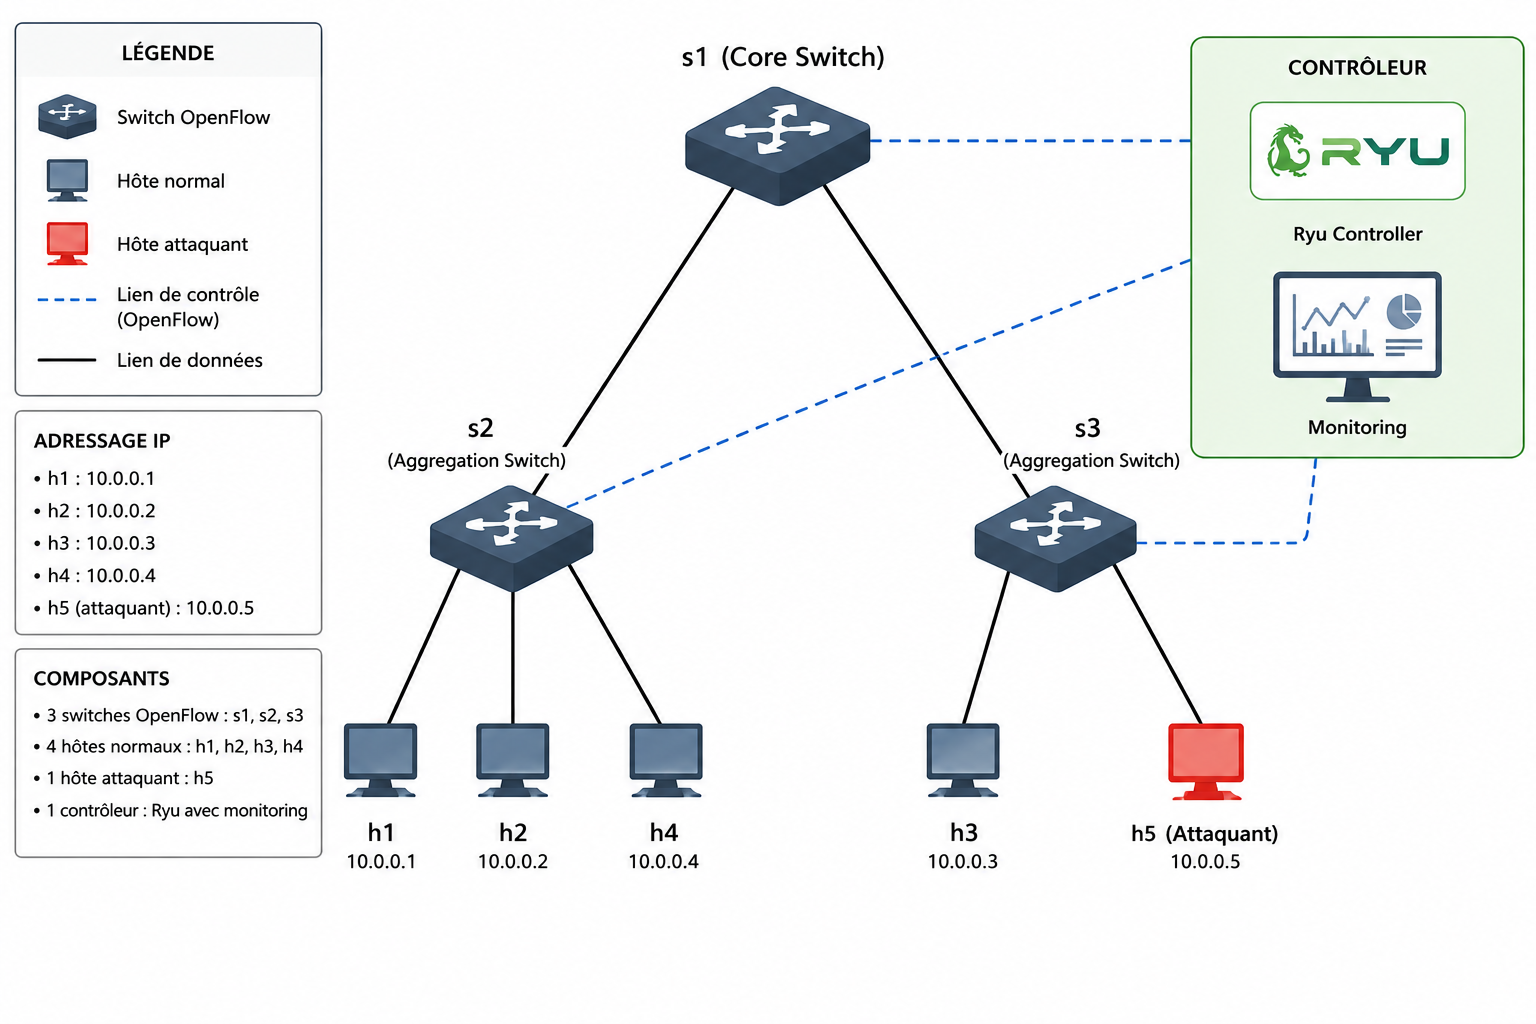
\includegraphics[width=0.8\textwidth]{images/topo_arbre.png}
\captionof{figure}{Exemple de topologie en arbre utilisée pour les tests}

\subsection{Exemple de séquence d'exécution}

Un scénario type se déroule en quatre temps. D’abord, la topologie est lancée avec un contrôleur Ryu et un ensemble d’hôtes de test. Ensuite, un trafic normal est établi entre plusieurs hôtes afin de constituer une ligne de base. Puis une attaque est déclenchée depuis l’hôte malveillant vers une cible choisie, ce qui permet d’observer l’évolution des métriques réseau et de la charge du contrôleur. Enfin, l’attaque est arrêtée pour vérifier le retour à un comportement normal.

Cette séquence rend possible la comparaison directe des métriques avant et après attaque, tout en produisant un jeu de données exploitable pour l’entraînement et l’évaluation du modèle.

\section{Résultats et discussion}\label{sec:results}

\subsection{Protocole expérimental}

L’évaluation du système proposé a été réalisée dans l’environnement expérimental décrit précédemment, reposant sur Mininet, Open vSwitch et le contrôleur Ryu instrumenté. Le pipeline complet, depuis la génération de trafic jusqu’à l’apprentissage, a été automatisé à l’aide du script \texttt{run\_full\_experiment.py}, garantissant la reproductibilité des expériences.

Le dataset final est constitué de plusieurs sessions d’exécution incluant des phases de trafic normal et des phases d’attaque. Après prétraitement, le jeu de test contient 3\,783 flux réseau, dont 2\,066 flux légitimes et 1\,717 flux malveillants. Ces données sont strictement disjointes de celles utilisées pour l’entraînement, ce qui permet une évaluation robuste des performances en généralisation.

Les attaques simulées couvrent plusieurs classes représentatives des menaces SDN, notamment les attaques par déni de service (ICMP flood, TCP SYN flood, UDP flood), les scans de ports et les attaques spécifiques au plan de contrôle telles que la surcharge \textit{Packet-In}. Cette diversité constitue un élément clé, car elle permet d’évaluer la capacité du modèle à capturer des comportements hétérogènes, en cohérence avec les scénarios étudiés dans la littérature récente sur les IDS SDN.

\subsection{Performances globales du modèle}
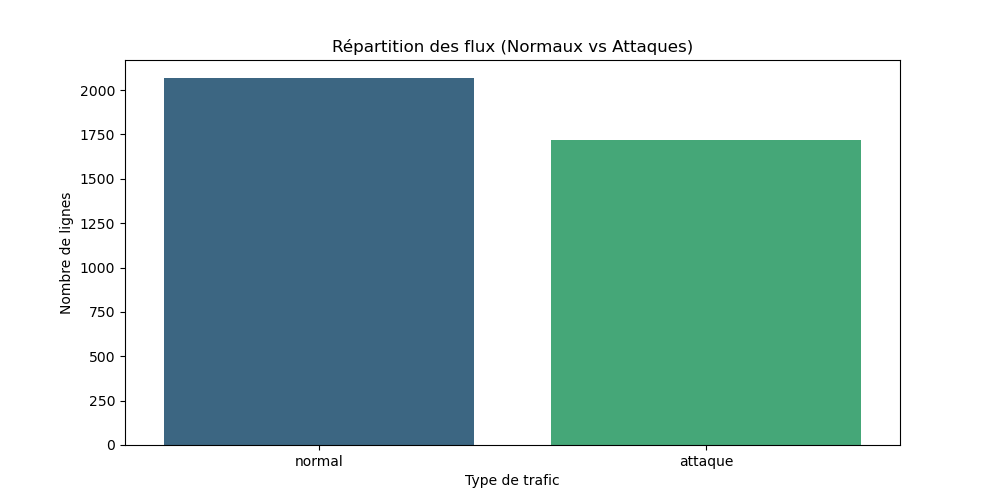
\includegraphics[width=0.8\textwidth]{images/repartition_trafic.png}
\captionof{figure}{Répartition du trafic réseau}

Le modèle Random Forest atteint une accuracy globale de 84,5\%, ce qui constitue un résultat satisfaisant au regard de la simplicité du modèle et de la diversité des scénarios considérés. Cette performance est cohérente avec les travaux existants montrant que les méthodes d’ensemble offrent un compromis pertinent entre coût computationnel et capacité de généralisation pour la détection d’attaques volumétriques en environnement SDN.

Cependant, dans un contexte de détection d’intrusions, l’accuracy seule est insuffisante. Les métriques de précision et de rappel sont particulièrement critiques, notamment pour la classe \textit{attaque}. Le modèle atteint une précision de 83\% et un rappel de 83\%, traduisant un compromis équilibré entre détection des comportements malveillants et limitation des fausses alertes.

Le score F1, égal à 0,83 pour les attaques et 0,86 pour le trafic normal, confirme la cohérence globale du modèle. Ces résultats indiquent que l’approche parvient à capturer des motifs discriminants dans les caractéristiques statistiques des flux, en particulier pour les attaques générant des variations marquées de débit ou de durée.

\subsection{Analyse des erreurs}

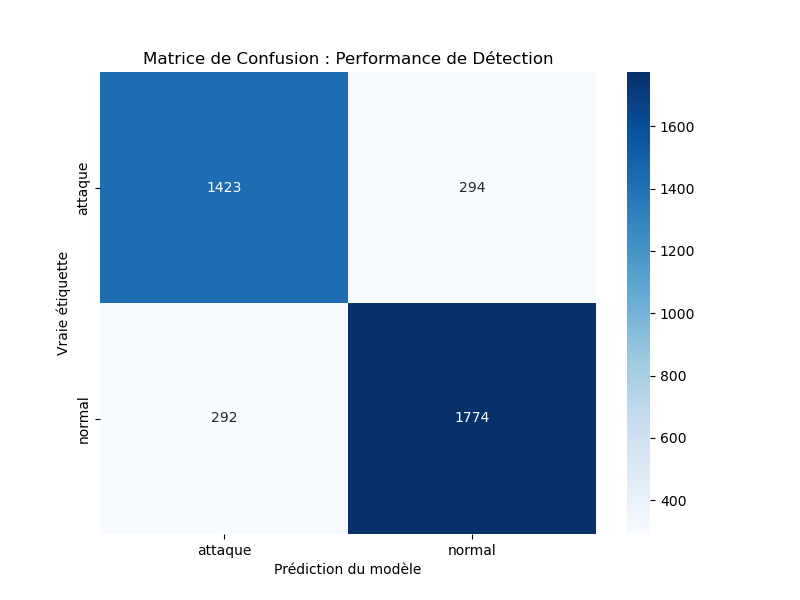
\includegraphics[width=0.8\textwidth]{images/matrice_confusion.png}
\captionof{figure}{Matrice de confusion du modèle Random Forest}

L’analyse de la matrice de confusion met en évidence les limites actuelles du système. Sur les 1\,717 attaques présentes dans le jeu de test, 1\,423 sont correctement détectées, tandis que 294 ne le sont pas. Ces faux négatifs constituent le principal point faible du modèle, car ils correspondent à des attaques non détectées, ce qui représente un risque critique dans un système de détection d’intrusions.

Une analyse plus fine suggère que ces erreurs sont principalement liées à des attaques de faible intensité ou à des comportements proches du trafic normal. En particulier, les attaques de type \textit{low-and-slow}, ainsi que certains scans furtifs, produisent des signatures statistiques difficilement distinguables du trafic légitime. Ce phénomène met en évidence une limite inhérente aux approches basées uniquement sur des caractéristiques agrégées.

Du côté des faux positifs, 292 flux normaux sont incorrectement classés comme malveillants. Bien que moins critiques en termes de sécurité, ces erreurs peuvent engendrer une surcharge opérationnelle et réduire la confiance dans le système.

Dans un contexte opérationnel, ce compromis a un impact direct sur la réponse du contrôleur SDN. Un faux négatif signifie qu’une attaque active n’est pas détectée et peut continuer à saturer le plan de contrôle sans alerte. À l’inverse, un faux positif déclenche une alerte inutile, ce qui augmente la charge de supervision mais ne compromet pas immédiatement la disponibilité du réseau. Dans une mise en production, il serait donc préférable de privilégier le rappel sur la classe attaque, quitte à accepter davantage de fausses alertes.

Ces résultats illustrent le compromis classique entre précision et rappel en détection d’intrusions. L’ajustement de ce compromis, par exemple via le réglage des hyperparamètres ou l’utilisation de techniques de calibration, constitue une piste d’amélioration importante.

\subsection{Importance des caractéristiques}

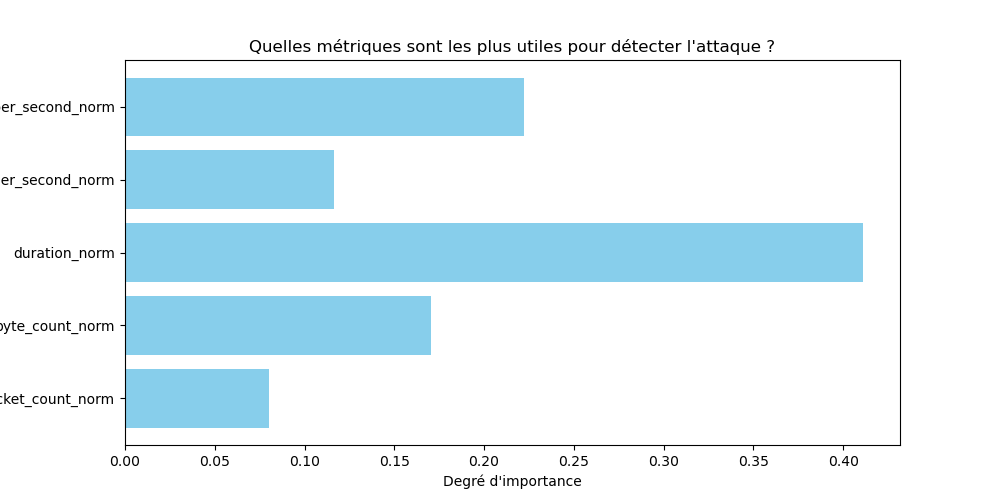
\includegraphics[width=0.8\textwidth]{images/importance_metriques.png}
\captionof{figure}{Importance des caractéristiques}

L’analyse de l’importance des variables montre que la durée des flux (\textit{duration}) est la caractéristique la plus discriminante, avec une contribution de 41\%. Elle est suivie par \textit{packets\_per\_second} (22\%), \textit{byte\_count} (17\%), \textit{bytes\_per\_second} (11\%) et \textit{packet\_count} (8\%). Cette hiérarchie confirme que les dimensions temporelles et de débit portent l’essentiel du signal discriminant.

Cette dominance s’explique par le fait que les attaques simulées, en particulier les attaques DoS, génèrent des flux atypiques en termes de temporalité et d’intensité. À l’inverse, un trafic normal intensif, tel qu’un transfert volumineux ou une sauvegarde, peut produire des signatures proches de celles d’un flood, ce qui explique une partie des erreurs observées.

Les variables de débit, telles que \textit{packets\_per\_second} et \textit{bytes\_per\_second}, jouent également un rôle significatif, confirmant que les dynamiques temporelles sont plus informatives que les volumes absolus.

Toutefois, cette forte dépendance à un nombre restreint de caractéristiques constitue une limite importante. Elle peut rendre le modèle vulnérable à des attaques adaptatives capables d’imiter les distributions statistiques dominantes. Ce phénomène est bien documenté dans la littérature sur les attaques adversariales en cybersécurité.

L’enrichissement du jeu de caractéristiques apparaît donc essentiel, notamment par l’intégration de métriques temporelles avancées, de corrélations inter-flux ou de descripteurs comportementaux plus complexes.

\subsection{Lecture qualitative du choix de modèle}

Le choix du Random Forest correspond à un compromis pragmatique. Par rapport à des architectures profondes de type CNN-LSTM, le modèle reste plus léger, plus simple à déployer dans le contrôleur et plus rapide à l’inférence. En revanche, il modélise moins bien les dépendances temporelles fines, ce qui le rend moins adapté aux attaques discrètes de type \textit{low and slow}. Cette limite justifie l’exploration future de modèles hybrides, combinant détection rapide et analyse séquentielle plus riche.

\subsection{Apport de l’environnement expérimental}

L’un des apports majeurs de ce travail réside dans la conception d’un environnement expérimental complet et reproductible. Contrairement à de nombreuses approches reposant sur des datasets statiques, notre méthode permet de générer dynamiquement des données dans un environnement contrôlé mais réaliste.

L’intégration d’un contrôleur Ryu instrumenté permet une collecte fine des métriques réseau, tandis que le générateur d’attaques modulaire offre une grande flexibilité dans la définition des scénarios. La labellisation automatique, basée sur le contexte d’exécution, constitue un avantage significatif en réduisant les biais humains et en améliorant la cohérence des annotations.

Cette infrastructure expérimentale constitue une base solide pour l’évaluation comparative de différentes approches de détection, et peut être étendue pour intégrer de nouveaux types d’attaques ou de nouvelles métriques.

\subsection{Limites et menaces à la validité}

Malgré les résultats encourageants, plusieurs limites doivent être discutées.

Tout d’abord, l’environnement Mininet, bien que réaliste, reste une émulation. Les performances observées peuvent différer dans des environnements de production caractérisés par des volumes de trafic plus importants et des comportements plus complexes.

Ensuite, le dataset utilisé, bien que diversifié, reste de taille modérée. Certaines classes d’attaques, notamment celles spécifiques au plan de contrôle, sont sous-représentées, ce qui peut introduire un biais dans l’apprentissage et limiter la capacité de généralisation.

Par ailleurs, la représentation des flux repose sur des caractéristiques agrégées, ce qui ne permet pas de capturer les dynamiques temporelles fines. Des modèles séquentiels, tels que les réseaux récurrents ou les approches basées sur des fenêtres temporelles, pourraient mieux modéliser ces dépendances.

Enfin, la formulation du problème en classification binaire simplifie l’analyse mais limite la capacité du système à différencier les types d’attaques, ce qui serait pourtant essentiel pour une réponse automatisée adaptée.

\subsection{Vers une détection en temps réel}

L’architecture actuelle repose en partie sur un traitement différé des données. Toutefois, les mécanismes implémentés dans le contrôleur Ryu permettent d’envisager une évolution vers une détection en flux continu.

Dans cette perspective, les statistiques OpenFlow peuvent être considérées comme un flux de données $\{\mathbf{x}_t\}_{t \geq 0}$, où chaque observation est traitée en temps quasi réel par le modèle. Une telle approche nécessite une optimisation des temps d’inférence ainsi qu’une gestion efficace du débit de données.

L’intégration dans une architecture de \textit{stream processing}, reposant par exemple sur des systèmes de files de messages ou de traitement distribué, permettrait de découpler la collecte, le traitement et la décision. Cette évolution ouvrirait également la voie à des approches d’apprentissage en ligne, capables d’adapter dynamiquement le modèle face à l’évolution des menaces.

\medskip

Dans l’ensemble, les résultats obtenus démontrent la pertinence de l’approche proposée pour la détection d’attaques dans des environnements SDN. Ils mettent également en évidence des axes d’amélioration clairs, tant au niveau des caractéristiques utilisées que de l’architecture de traitement. Le système constitue ainsi une base prometteuse pour le développement d’un IDS SDN intelligent, évolutif et adapté à des contextes opérationnels.













\section{Conclusion et perspectives}\label{sec:conclusion}

Dans cet article, nous avons proposé \textit{Cybernet IA}, un système de détection d’intrusions dédié aux environnements SDN, reposant sur une approche d’apprentissage supervisé basée sur l’algorithme Random Forest. En nous appuyant sur une architecture expérimentale complète intégrant Mininet, Open vSwitch et le contrôleur Ryu, nous avons conçu un pipeline de bout en bout permettant la collecte, la transformation et l’exploitation de données réseau dans un cadre reproductible et représentatif d’un environnement SDN réel.

Les résultats expérimentaux obtenus démontrent la pertinence de l’approche proposée pour la détection d’attaques affectant le plan de contrôle, notamment les attaques de type déni de service et les activités de scan. Avec une précision et un rappel équilibrés autour de 83\%, le modèle parvient à capturer efficacement des motifs discriminants à partir de caractéristiques statistiques simples extraites des flux OpenFlow. L’analyse des variables confirme par ailleurs le rôle structurant de certaines métriques agrégées, en particulier la durée des flux et les indicateurs de débit, dans le processus de décision.

Au-delà des performances quantitatives, une contribution majeure de ce travail réside dans la conception d’un environnement expérimental modulaire, automatisé et extensible. Contrairement à de nombreuses approches reposant sur des jeux de données statiques, la plateforme proposée permet de générer dynamiquement des scénarios d’attaque variés, de produire des données labellisées de manière cohérente et de garantir la reproductibilité des expériences. Cette infrastructure constitue ainsi un outil pertinent pour l’évaluation comparative de méthodes de détection dans des conditions contrôlées.

Néanmoins, plusieurs limites doivent être prises en compte. D’une part, la dépendance du modèle à un nombre restreint de caractéristiques, notamment la durée des flux, peut affecter sa robustesse face à des attaques plus sophistiquées cherchant à imiter le trafic légitime. D’autre part, bien que l’intégration avec le contrôleur SDN soit amorcée, l’architecture actuelle repose encore en partie sur un traitement différé des données, ce qui limite la réactivité du système dans des contextes opérationnels contraints.

Ces limites ouvrent plusieurs perspectives de recherche. Une première direction consiste à faire évoluer l’architecture vers un traitement en flux continu (\textit{streaming}), permettant une détection en temps réel directement au niveau du contrôleur SDN. Une telle évolution implique l’intégration de mécanismes d’inférence à faible latence ainsi que l’exploration de paradigmes d’apprentissage incrémental capables de s’adapter dynamiquement à l’évolution du trafic réseau.

Une seconde piste concerne l’enrichissement du jeu de caractéristiques, notamment par l’intégration de descripteurs temporels ou contextuels permettant de mieux capturer les comportements séquentiels des attaques. Dans cette optique, l’étude de modèles capables d’exploiter explicitement la dimension temporelle, tels que les approches basées sur les séries temporelles ou les architectures hybrides, constitue une direction prometteuse.

Enfin, une évaluation comparative approfondie avec d’autres méthodes d’apprentissage, telles que les approches de type \textit{gradient boosting} ou les modèles hybrides combinant classification supervisée et détection d’anomalies, permettrait de mieux situer les performances de la solution proposée et d’identifier des axes d’amélioration complémentaires.

Ainsi, ce travail s’inscrit dans une démarche plus large visant à rapprocher les techniques d’intelligence artificielle et les infrastructures réseaux programmables, en proposant des solutions concrètes pour renforcer la sécurité des architectures SDN. À terme, ces contributions pourraient participer à l’émergence de contrôleurs intelligents capables d’intégrer nativement des mécanismes d’auto-protection adaptatifs face aux menaces émergentes.
\bibliographystyle{plain}
\bibliography{references}

\end{document}